\chapter{Projekt}
Rodział czwarty opisuje projekt systemu repozytorium testów funkcjonalnych. Składa się z trzech części. Część pierwsza opisuje ogólną architekturę systemu. Druga część specyfikuje warstwy systemu to jest warstwa aplikacji internetowej i warstwa usługi internetowej. Trzecia część opisuje poszczególne moduły systemu.

\section{Architektura}
Aplikacja stworzona będzie w architekturze klient-serwer. Interfejs użytkownika zrealizowany będzie w technologii aplikacji internetowych, tak by dostęp do repozytorium nie wymagał instalacji i był dostępny na różnych platformach. Dodatkowo stworzona zostanie usługa internetowa (ang. web service), tak by umożliwić zintegrowanie aplikacji z zewnętrznymi aplikacjami dzięki czemu możliwa będzie automatyzacja kluczowych procesów. Utrwalanie danych relizowane będzie w relacyjnej bazie danych poprzez moduł odwzorowujący obiektową architekturę systemu informatycznego na bazę danych.

Aplikacja zostanie napisana w języku JAVA. Język ten jest obecnie najczęściej spotykanym językiem w zagadnieniach korporacyjnych. Posiada rozwinięte wsparcie społeczności i rozbudowane funkcjonalności wbudowane, jak i rozwijane przez zewnętrznych kontrybutorów. 
\begin{figure}[h]
\centerline{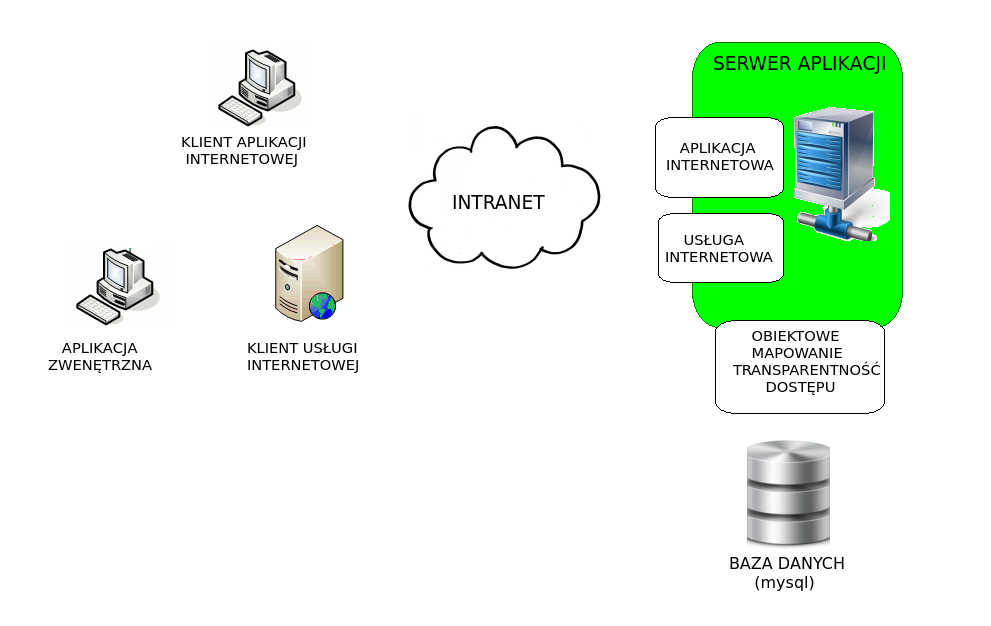
\includegraphics[scale=0.45]{img/architektura.png}}
\caption{Architektura systemu}
\label{fig:architektura}
\end{figure}


%<< Diagram fizyczny >>       

%<< Diagram komponentów >>

%Komponent zarządzanie użytkownikami

%Komponent Definicji 

%Komponent wykonania testów

%Komponent danych dodatkowych
\section{Warstwy}
W projektowanym systemie można wyróżnić dwie warstwy poprzez które klient może komunikować się w systemie. Pierwsza warstwa to jest aplikacja internetowa przewidziana jest do interakcji człowiek-komputer. Druga warstwa, to jest usługa internetowa przewidziana jest dla interakcji komputer-komputer. Kolejne dwa podrozdziały opisują specyfikę każdej z warstw.
\subsection{Warstwa aplikacji internetowej}
Dostęp poprzez aplikację internetową jest podstawowym źródłem interakcji użytkownika w projektowanej aplikacji. Celem rozdzielenia poszczególnych odpowiedzialności modułów oprogramowania, użyty zostanie wzorzec Model-Widok-Kontroler. Zakłada on wydzielenie trzech warstw:
\begin{enumerate}
  \item Model - odpowiedzialny za pobranie i enkapsulacje danych;
  \item Widok - odpowiedzialny za wyświetlenie sformatowanej treści. Język stosowany w widoku powinien pozwalać na swobodne osadzanie treści języka końcowego (w tym przypadku HTML), powinien on być dostosowany do edycji przez osoby nie posiadające wiedzy na temat języku programowania;
  \item Kontroler - odpowiedzialny za skoordynowanie pobrania danych, przetworzenia ich za pomocą serwisów i przesłanie danych do widoku.
\end{enumerate}

Język JAVA oferuje technologie objęte zdefiniowanym standardem które pozwalają tworzyć aplikacje internetowe z wykorzystaniem wzorca Model-Widok-Kontroler. Zaprezentowana aplikacja stworzona zostanie w oparciu o technologię Java Server Faces jej implementacje Mojarra wzbogaconą o komponenty PrimeFaces.

Java Server Faces jest jednym ze standardów tworzenia aplikacji internetowych w języku JAVA\cite{jsfRef}. Główne założenia standardu to:
\begin{enumerate}
  \item Łatwość tworzenia części klienckiej (widoku) w oparciu o strukturę komponentową. Udostępnione są standardowe komponenty (takie jak na przykład formularz, pole tekstowe);
  \item Możliwość zagnieżdżania struktury dokumentu, pozwalająca na minimalizację redundancji po stronie szablonu strony internetowej; 
  \item Zdefiniowany standard dostęp z widoku do danych po stronie serwera;
  \item Zapewnienie trwałości stanu danych pomiędzy żądaniami w obrębie sesji klienta;
  \item Część serwerowa oparta jest na ziarnach (ang. JavaBeans), posiada wsparcie dla walidacji zarówno po stronie klienckiej jak i serwerowej;
\end{enumerate}

W technologii Java Server Faces rola Kontrolera rozdzielona jest na pliki szablonu strony i ziarna zarządzające po stronie serwera. W plikach szablonu osadzone są instrukcję które wprost pobierają dane z kontrolera i wykonują na nim akcje.

Standard Java Server Faces posiada wiele implementacji. W tworzonej aplikacji użyta została implementacja PrimeFaces\cite{primeFaces}. PrimeFaces jest rozwijany jako otwarty projekt. Implementacja ta rozszerza standard o własne komponenty, uproszcza również sposób komunikacji klient serwer poprzez AJAX (asynchroniczna komunikacja poprzez język JavaScript)

\subsection{Warstwa usługi internetowej}



Jednym ze standardów komunikacji między aplikacjami jest komunikacja poprzez usługę internetową, dla której istnieje wiele technologii. W niniejszej pracy użyta zostanie technologia REST. REST zakłada iż deklaracja działania które klient zamierza osiągnąć po stronie serwera określona poprzez zasób. Odwołanie do zasobu składa się z:
\begin{enumerate}
  \item URI czyli adres internetowy określa adres zasobu do którego odwołuje się klient;
  \item  typ metody HTTP (zgodnie z HTTP/1.1) określa jakie działanie ma być podjęte na zasobie (wyświetlenie, dodanie, modyfikacja, usunięcie).
\end{enumerate}

Zgodnie ze specyfikacją HTTP/1.1 możemy wyróżnić następujące metody i oczekiwany rezultat po stronie serwerowej:

\renewcommand\multirowsetup{\centering\arraybackslash}
\begin{longtable}{|c|c|}
\hline
\textbf{metoda} & \textbf{mapowanie na akcje} \\ \hline
GET & Wyświetlenie, pobranie zasobu \\ \hline
PUT & Stworzenie zasobu \\ \hline
POST & Modyfikacja zasobu \\ \hline
DELETE & Usunięcie zasobu \\ \hline
OPTIONS, TRACE, HEAD & nie używane \\ \hline

\caption{Metody HTTP/1.1 \cite{http}}
\end{longtable}

Poprzez usługę internetową możliwe będzie wykonanie następujących akcji:
\begin{enumerate}
  \item dodanie wymagania;
  \item pobrania listy przypadków testowych do wykonania dla użytkownika;
  \item aktualizacji wykonania przypadku testowego.
\end{enumerate}
Pierwszy punkt pozwala na integracje z aplikacją przechowującą wymagania. Punkt drugi i trzeci pozwala na integracje z zewnętrznymi aplikacjami do wykonywania testów. W szczególnym przypadku poprzez stworzenie fikcyjnego użytkownika np. automatyzacja, można zintegrować repozytorium z modułem wykonującym testy automatycznie.


\section{Moduły aplikacji}
Funkcjonalności realizowane przez aplikację możemy podzielić na logicznę moduły. Opis poszczególnych modułów czytelnik znajdzie w kolejnych podrozdziałach.
\begin{figure}[h]
\centerline{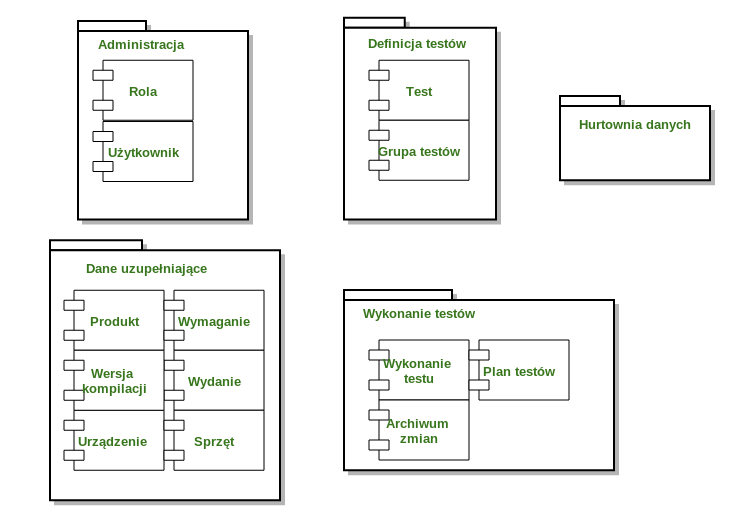
\includegraphics[scale=0.5]{img/komponenty.png}}
\caption{Moduły systemu}
\label{fig:moduly}
\end{figure}

\subsection{Moduł administracji}

Moduł ten skupia wszelkie funkcjonalności związane z zarządzaniem użytkownikami w systemie. Odpowiada za tworzenie i edycję użytkowników. Każdy użytkownik posiada takie dane jak login, adres e-mailowy, hasło jak również przypisaną rolę.

Możemy wyróżnić kilka ról użytkowników. Rola określa jakie uprawnienia otrzymuje zalogowany użytkownik i określa widok ekranu początkowego. Każda z ról posiada charakterystyczne cechy które pokrywają role użytkowników w procesie testowania oprogramowania: menedżer testów, lider testów, inżynier testów, specjalista środowiska do testów, specjalista konfiguracji testowej \cite{peopleWare}. Poniżej zaprezentowany zostanie opis poszczególnych ról.
\begin{enumerate}
  \item Administrator --  zarządza użytkownikami w systemie. Administrator tworzy użytkowników i nadaje im uprawnienia.
  \item Koordynator testów -- tworzy przypadki testowe, grupy testów i plany testów. Rola ta odpowiedzialna jest za treści merytoryczne repozytorium. Użytkownik odpowiada za utrzymanie testów, aktualizację ich, pokrycie funkcjonalności. 
  \item Obsługa techniczna -- rola ta odpowiedzialna jest za zapewnienie odpowiedniego środowiska dla testerów, konserwacje i naprawę fizycznych defektów. Użytkownik ten przypisany jest do konkretnych wykonań scenariuszy, instaluje początkowe środowisko, wymagane wersje oprogramowania, naprawia usterki sprzętowe.
  \item Lider testów -- wspiera zespół w wykonywaniu planu testów testowego. Służy swoją wiedzą i doświadczeniem przy podziale prac i podczas pojawiających się problemów. Posiada władzę decyzyjną przy zakwalifikowaniu testu jako nie udanego. Lider przypisuje testerów do testów.
  \item Tester --  wykonuje przypisane do niego przypadki testowe. Odznacza stan testów i zgłasza napotkane problemy.
  \item Pośrednik (ang. liaison) --  Odpowiedzialny jest za komunikacje zespołu testów z zespołem programistycznym. Posiada wgląd do aktualnie wykonywanych testów i konfiguracji. Jego zadaniem jest rozwiązywanie problemów związanych z jego macierzystym produktem. Pomaga zakwalifikować problem powstały podczas testów, szczególnie na początku testów produktu, zespół testerki może nie posiadać wystarczającej wiedzy i błędnie kwalifikować obserwowane rezultaty jako błąd produktu. Pośrednik proponuje również tymczasowe rozwiązania które pozwalają obejść problemy wynikające z błędów w oprogramowaniu, które naprawione będą dopiero podczas przyszłych wersji oprogramowania, tak by proces testowania mógł przebiegać nieprzerwanie.
\end{enumerate}
  
\subsection{Moduł definicji}

Moduł ten jest odpowiedzialny za definicję podstawowych jednostek systemu czyli: testów, grup testów i planów testów. 

Podstawową jednostą aplikacji jest przypadek testowy. Składowe przypadku testowego przedstawione są w tabeli \ref{tab:test}; 
\begin{longtable}{| p{6cm}  | p{10cm} |}
 \hline 
\textbf{Nazwa elementu} & \textbf{Opis}  \\ \hline
\endfirsthead
\multicolumn{2}{c}%
{\tablename\ \thetable\ -- \textit{Kontynuacja}} \\
\hline
\textbf{Nazwa elementu} & \textbf{Opis}  \\
\hline
\endhead
\hline \multicolumn{2}{r}{\textit{Kontynuacja na następnej stronie}} \\
\endfoot
\endlastfoot
  identyfikator & jednoznacznie identyfikujący test, unikatowy ciąg znaków \\ \hline
  tytuł & tytuł testu \\ \hline
  abstrakt &  opis testu, jego kluczowe założenia, tematyka i tło określające test \\ \hline
  grupy urządzeń & Do jednej grupy urządzeń może być przypisane jedno lub więcej urządzeń (w przypadku gdy dana funkcjonalność adresowana jest na więcej niż jedno urządzenie danego typu). Podczas wykonania testu należy jednak określić którego urządzenia z grupy należy użyć (wybrać jedno)\\ \hline
  stan wejściowy konfiguracji & Lista sprzętów i ich stanów  które są wymagane do wykonania testu. Dla każdego ze stanów można zdefiniować warunek określający dla jakich konfiguracji grup urządzeń stan ma zajść \\ \hline
   scenariusz &  lista kroków do wykonania wraz z oczekiwanymi rezultatami \\ \hline
    wymagania & lista wymagań które są weryfikowane poprzez wykonanie testu \\ \hline
    estymowany czas & estymowany czas potrzebny do wykonania przypadku testowego \\ \hline
     stan początkowy produktów & stan początkowy poszczególnych produktów który musi być spełniony. Dla każdego ze zdefiniowanych stanów możliwe jest przypisanie warunku który określa dla jakiej konfiguracji grup urządzeń stan ma zajść \\ \hline
     liczba wariacji & liczba możliwych alternatywnych przebiegów przypadku testowego (w zależności od doboru urządzeń) \\ \hline 
 \caption{ Składowe przypadku testowego}
 \label{tab:test}
\end{longtable}


Przypadki testowe wchodzą w skład grup testów. Hierarchia ta ma drzewiastą strukturę co oznacza iż grupy mogą być zagnieżdżone. Grupy powinny agregować testy które posiadają podobną charakterystykę. Na przykład testują te same funkcjonalności, wymagają podobnej konfiguracji, urządzeń, dokumentacji. Testy funkcjonalne i niefunkcjonalne nie powinny znajdować się w tej samej grupie. Składowe grupy testów przedstawione są w tabeli \ref{tab:grupaTestow}

\begin{longtable}{| p{6cm}  | p{10cm} |}
 \hline \hline
\textbf{Nazwa elementu} & \textbf{Opis}  \\ \hline
  identyfikator & jednoznacznie identyfikujący grupę, unikatowy ciąg znaków \\ \hline
  identyfikator rodzica & grupy mogą przybierać postać drzewiastą \\ \hline
  tytuł & tytuł grupy testowej \\ \hline
  opis & opis grupy testowej, określający jakiego typu testy powinny znaleźć się w grupie \\ \hline
 \caption{ Składowe grupy testów}
 \label{tab:grupaTestow}
\end{longtable}


\subsection{Moduł danych uzupełniających}

Definicja testów przez swoją złożoność i potrzebę pełnej specyfikacji wymaga pewnych danych dodatkowych które muszą zostać zdefiniowane w aplikacji. Repozytorium przeznaczone jest dla systemów wiele-wydaniowych i wspierany jest inkrementacyjny model wytwarzania oprogramowania.

Pierwszym krokiem jest zdefiniowanie produktów wchodzących w skład systemu który poddany zostanie testom. System w kontekście aplikacji jest to zbiór zintegrowanych produktów które współdziałając oferują określoną funkcjonalność z perspektywy klienta.

W celu wsparcia inkrementacyjnego modelu wytwarzania oprogramowania w aplikacji istnieją takie elementy jak ,,wydanie produktu'' i ,,wersja produktu'' która wchodzi w skład wydania. Poprzez wersje produktu rozumiany jest konkretny skompilowany stan komponentów systemu. Wersja systemu powinna być jednoznacznie identyfikowalna ponieważ stanowi linie bazową. Na podstawie porównania dwóch poprzedzających się wersji można określić kiedy został wprowadzony błąd regresji. Wydania produktu są to wersje widoczne z poziomu klienta końcowego, w ich skład najczęściej wchodzi wiele wersji.

W ramach wydań produktów definiowane są wymagania. Wymaganie powinno być jasno zdefiniowane tak by możliwe było zweryfikowanie spełnienia wymagania przez oprogramowanie. Na podstawie wymagań tworzone są przypadki testowe.

Drugą charakterystyką aplikacji jest wsparcie dla systemów dedykowanych na wiele urządzeń. Aplikacje umożliwia więc przechowywanie informacji o urządzeniach. Definicja urządzenia powinna zawierać dane podstawowe takie jak nazwa, dostawca, zdjęcie jak i referencję do kompletnej dokumentacji na temat urządzenia. Dostęp do dokumentacji jest kluczowy podczas testów, szczególnie dla młodego stażem zespołu testującego.

W module definicji testów, podczas tworzenie przypadku testowego tworzone są grupy urządzeń. W skład grupy może wejść jedno lub więcej urządzeń, przy czym podczas wykonania przypadku testowego należy wybrać tylko jedno urządzenie dla każdej z grup. Konfiguracja wybranych urządzeń determinuje i modyfikuje końcową treść przypadku testowego. Od tego które urządzenia zostały wybrane mogą zależeć poszczególne kroki, stany początkowe produktów i wymagany sprzęt. Aplikacja repozytorium udostępnia sposób definiowania warunków dla wcześniej wspomnianych elementów. Warunek określa iż dany element jest ważny (wchodzi w skład definicji przypadku testowego) wtedy i tylko wtedy gdy dla określonej grupy urządzeń wybrane zostało określone urządzenie.

Jednym z elementów wykonania testów funkcjonalnych jest instalacja środowiska do wykonania testów. Instalacja składa się z kilku elementów:
\begin{itemize}
  \item dostarczenie i zainstalowanie sprzętu wymaganego do wykonania testów (przykładowo może to być symulator fal radiowych, sejf automatyczny, kabel ethernet, komputer stacjonarny);
  \item instalacja platformy do wykonania testów (systemy operacyjne, środowiska uruchomieniowe, modyfikacji systemów, bios, maszyny wirtualne);
  \item instalacja oprogramowania w wersji zgodnej z planem testów.
\end{itemize}

\subsection{Moduł wykonania }

Moduł ten przechowuje informacje o realizowanych planach testowych, testach oczekujących do wykonania i historie wykonywanych przypadków testowych.

Pierwszym krokiem jest utworzenie planu testów. Plan testów określa ramy testów, definiuje co i dlaczego powinno zostać przetestowane, określa konfigurację środowiska testowego. Specyfikacja planu testów znajduje się w tabeli \ref{tab:planTestow}

\begin{longtable}{| p{6cm}  | p{10cm} |}
 \hline 
\textbf{Nazwa elementu} & \textbf{Opis}  \\ \hline
\endfirsthead
\multicolumn{2}{c}%
{\tablename\ \thetable\ -- \textit{Kontynuacja}} \\
\hline
\\textbf{Nazwa elementu} & \textbf{Opis}  \\
\hline
\endhead
\hline \multicolumn{2}{r}{\textit{Kontynuacja na następnej stronie}} \\
\endfoot

\endlastfoot
  identyfikator & jednoznacznie identyfikujący plan, unikatowy ciąg znaków \\ \hline
  tytuł & tytuł plan \\ \hline
  opis & opis planu testowego \\ \hline
  wymagania & lista wymagań których spełnienie zostanie zweryfikowane podczas przeprowadzania testów \\ \hline
  urządzenia & lista urządzeń dostępnych podczas testów \\ \hline
  wersja systemu & wersja systemu która będzie wdrożona podczas testowania  \\ \hline
 \caption{ Składowe planu testów}
 \label{tab:planTestow}
\end{longtable}

Po utworzeniu planu testowego należy przypisać do planu testy które mają zostać wykonane. Wyboru należy dokonać biorąc po uwagę potrzebę spełnienia planu przy określonych zasobach ludzkich, pokrycia wymagań i ograniczeń wynikających z dostępności sprzętu i urządzeń.

Plan testów określa jakie wymagania należy zweryfikować, jest to kluczowy aspekt podczas doboru przypadków testowych. Należy dobrać takie przypadki testowe które weryfikuję potrzebne wymagania. Na tym jednak dobór przypadków testowych nie powinien być zakończony. Należy pamiętać o potrzebie przeprowadzenia regresji. Fakt iż określona wersja systemu dostarcza pewne funkcjonalności nie oznacza iż poprzednio przetestowane funkcjonalności dalej działają poprawnie.

Podczas przypisania przypadku testowego do planu, należy go dookreślić w przypadku gdy posiada grupy urządzeń złożone z więcej niż jednego urządzenia. Oznacza to iż należy wybrać jedno i tylko jedno urządzenie dla każdej z grup. Wybór z jednej strony warunkowany jest dostępnymi zasobami sprzętowymi, a z drugiej strony powinien uwzględniać przetestowanie wszerz systemu dla różnych konfiguracji sprzętowych. Należy unikać w sytuacji w której nie zostaną wykonane testy na urządzeniach które są poprawne z perspektywy klienta.

Po dokonaniu pełnej definicji przypadku testowego, rozwiązywane są wszystkie warunki określone w takich elementach jak: stany produktu, kroki testu, warunki początkowe. Dla przypomnienia dla tych elementów można określić warunki które stanowią iż dany element wchodzi w skład przypadku testowego wtedy i tylko wtedy gdy dostępna jest konkretna konfiguracja sprzętowa (wybrane zostało konkretne urządzenie z grupy urządzeń). Schemat dla stanów produktów można przedstawić pseudokodem znajdującym się w listingu \ref{lst:doborWarunkow}.
\begin{figure}[h]
	\begin{codebox}
	\li \For{$stanProduktu$ \kw{in} $stanyProduktu$}
	\li \Do   
	\For{$warunek$ \kw{in} $warunkiDlaGrupUrzadzen$}
	\li \Do
	     \If $wybraneUrzadzenie  ==  preferowaneUrzadzenieDlaStanu$
	\li     \Then
	           $\proc{dodaj-stan-do-testu}(stanProduktu)$	         	         
	        \End	        
	\li  \End	 
	\li
	  \End
	  
	\end{codebox}
	\caption{ Algorytm doboru stanów produktu do przypadku testowego }
	\label{lst:doborWarunkow}
\end{figure}
\newpage

Rezultat wykonania przypadku testowego może przyjmować jedną wartość z podanych:
\begin{itemize}
   \item oczekujący - przypadek testowy oczekuje na przypisanie przez testera (każda osoba z zespołu może się przypisać);
   \item przypisany - przypadek testowy przypisany do testera (przypadek nie jest już widoczny w puli);
   \item zablokowany - przypadek testowy zablokowany przez błąd w innym przypadku, bądź poprzez niegotową konfigurację;
   \item rezultat pozytywny - wszystkie kroki scenariusza wygenerowały oczekiwane rezultaty;
   \item rezultat negatywny - przynajmniej jeden z kroków scenariusza wygenerował rezultat negatywny, lub testy eksploracyjne związane z przypadkiem testowym wygenerowały rezultat negatywny;
   \item nie możliwy do wykonania - przypadek niemożliwy do wykonania z przyczyny braku zasobów;
   \item wymagana analiza - podczas wykonywania przypadku testowego, wyniki poszczególnych kroków scenariusza nie dały jednoznacznej odpowiedzi. Wymagana jest konsultacja lidera i pośrednika (ang. \textit{liaisona}).
 \end{itemize} 

Po wykonaniu przypadku testowego, tester oznacza wynik wykonania przypadku testowego i w razie konieczności opisuje wnioski jako komentarz. Tester uzupełnia też realny czas poświęcony na wykonanie przypadku testowego.

\subsection{ Moduł hurtowni danych  }

Moduł ten odpowiedzialny jest za interpretacje danych istniejących w repozytorium. Przedstawiane są tutaj metryki i wykresy kluczowe z perspektywy lidera, koordynatora i kierownika testów.

Pierwszą z grup raportów jest wykres pokrycia wymagań na poziome definicji testów. Analiza pozwala określić które części wymagań nie są pokryte przez przypadki testowe.

Drugą grupą jest pokrycie wymagań na podstawie wykonania przypadków testowych. Pokrycia można analizować odpowiednio z poziomu pojedynczego planu testów, grupy testów i całego wydania systemu. Dane te dostarczają informacji na temat tego które z wymaganych obszarów zostały pokryte podczas rzeczywistych testów. Dzięki tym informacją kierownik zespołu testów może zaplanować zakres kolejnych planów testów.

Trzecia grupa dotyczy relacji pomiędzy urządzeniami a przypadkami testowymi. Analiza danych dostarczanych w tej grupie pozwala określić które urządzenia zostały już przetestowana a także które urządzenia należy dostarczyć i włączyć w przyszłych przypadkach testowych.

Czwarta grupa dotyczy procentowego stanu przypadków testowych. Analiza danych dostarczanych przez tą grupę pozwala określić czy wraz z czasem projektu zmniejsza się liczba znajdywanych defektów, określić procent testów zablokowanych i inne wnioski które mogą wpłynąć na zwiększenie efektywności zespołu testującego.



\chapter{Implementacja}

Rozdział 5 opisuje szczegóły implementacji zaprojektowanego rozwiązania. Rozdział ten podzielony został na cztery części: część pierwsza opisuje ogólną organizacje aplikacji, druga część opisuje model bazy danych, trzecia część opisuje implementacje części aplikacji internetowej, czwarta część opisuje implementacje usługi internetowej.

\section{Organizacja aplikacji}
Sekcja ta opisuje wysoko-poziomową strukturę aplikacji. W podrozdziałach przedstawione zostanie: środowisko uruchomieniowe na którym zaimplementowana została aplikacja oraz struktura plików i bibliotek w projekcie.
\subsection{Środowisko uruchomieniowe aplikacji}
Platforma korporacyjna języka JAVA (ang. \textit{JAVA Enterprise}) określa sposób tworzenia wielowarstowych systemów w tym języku. Poszczególne funkcjonalności udostępniane są poprzez komponenty.  Przykładowymi funkcjonalnościami oferowanymi przez platformę korporacyjną są: dostęp do bazy danych, serializacja danych do formatu XML, zarządzanie sesjami i transakcjami, autoryzacja i autentykacja, wstrzykiwanie zależności, funkcjonalność aplikacji internetowej, funkcjonalność usługi internetowej. Aplikacje tworzone w oparciu o platformę korporacyjną mogą być wdrażane transparentnie na różnych platformach docelowych.Specyfikacja platformy korporacyjnej JAVA określa również ścieżki i format plików konfiguracyjnych za pomocą których możliwa jest konfiguracja określonych funkcjonalności.

Środowisko które obsługuję programy oparte na platformie korporacyjnej nazywamy serwerem aplikacji. Jest to zrąb który udostępnia usługi i środowisko pozwalające uruchomiać i zarządzać aplikacjami w tym aplikacjami internetowymi. Zachowanie serwera aplikacji porównać można do wirtualnej maszyny dla uruchamianych aplikacji która transparentnie udostępnia określone usługi. Zgodnie ze specyfikacją platformy korporacyjnej serwer aplikacyjny musi udostępniać implementacje standardowych funkcjonalności i serwisów oferowanych przez tą platformę. 

Specyfikacja platformy korporacyjnej JAVA określa interfejsy dla komponentów. Serwery aplikacyjne dostarczają natomiast referencyjnych implementacji, przy czym implementacja może rozszerzyć zbiór funkcjonalności o własne funkcjonalności specyficzne dla dostawcy. Podczas życia produktu, istnieje możliwość migracji do innej implementacji serwera aplikacji lub nadpisania implementacji określonej technologii na implementacje innego dostawcy. Tego typu migracje mogą nastąpić transparentnie w przypadku gdy implementacja kliencka korzysta jedynie z funkcjonalność oferowanych przez interfejs. Korzystanie z rozwiązań specyficznych dla dostawcy powoduje konieczność migracji ich na analogiczne rozwiązania dla nowego dostawcy lub stworzenia własnego rozwiązania w przypadku gdy nowy dostawca nie udostępnia wymaganej funkcjonalności.

Istnieje wiele implemetacji serweru aplikacji dla platformy korporacyjnej języka JAVA. Podczas implementacji repozytorium użyty został serwer aplikacji Glassfish. Serwer aplikacji Glassfish, jest to referencyjna, otwarta i bezpłatna implementacja serwera aplikacji stworzona przez firmę Oracle. 

W stworzonej aplikacji użyte zostały jedynie rozwiązania specyfikowane w interfejsach funkcjonalności platformy korporacyjnej. Oznacza to iż migracja na inny serwer aplikacji może odbyć się transparentnie.
\subsection{Struktura projektu}
Pliki źródłowe projektu zostały podzielone na sekcje tak by w sposób przejrzysty rozdzielić poszczególne elementy. Zastosowany podział przedstawiony został na rysunku \ref{fig:stukturaProjektu}. Stworzone zostały osobne katalogi dla: bibliotek, kodu źródłowego i docelowych artefaktów. Pliki kodu źródłowego podzielone zostały na: kod aplikacji i testy jednostkowe.

\begin{figure}[h!]

\dirtree{%
.1 lib \DTcomment{ lokalne biblioteki}.
.1 src.
.2 main.
.3 java \DTcomment{ kod źródłowy aplikacji }.
.3 resources \DTcomment{ pliki konfiguracyjne aplikacji }.
.3 webapp \DTcomment{ pliki dotyczące konfiguracji aplikacji internetowej }.
.2 test.
.3 java \DTcomment{ testy jednostkowe }.
.1 target \DTcomment{ zbudowane artefakty aplikacji }.
.1 pom.xml.
}
\caption{Organizacja plików projektu}
\label{fig:stukturaProjektu}
\end{figure}

Wszelkie zależności wymagane przez aplikacje rozwiązywane są poprzez narzędzie do automatycznego budowania projektów Maven. Maven poprzez konfiguracje zdefiniowaną w pliku pom.xml określa które biblioteki są wymagane przez aplikację i pobiera je podczas budowania aplikacji. Narzędzie to poprzez system wtyczek pozwala na zdefiniowanie celów budowania i wdrażania projektu. W zaimplementowanej aplikacji został zdefiniowany cel który: pobiera biblioteki zależne, kompiluje kod produkcyjny i kod testów jednostkowych, wykonuje wszystkie testy jednostkowe i w przypadku powodzenia instaluje archiwum aplikacji internetowej (ang. WAR) na serwerze aplikacji.


\section{Model bazy danych}
Glassfish dostarcza bibliotekę EclipseLink która spełnia standardy między innymi warstwy dostępu do danych (ang. JPA) i łączenia danych do i z formatu XML (JAXB). Na poziomie kodu aplikacji, struktura połączenia obiektów z bazą relacyjną jest rozwiązywana poprzez zastosowanie standardowych adnotacji. Zastosowania standardowych adnotacji zgodnych ze standardem JPA pozwala na transparentność dostawcy modułu mapującego relacyjną bazę danych. W przypadku zmiany dostawcy, migracja dotyka jedynie pewnych plików konfiguracyjnych które zawierają specyficzne ustawienia dla dostawcy (np. sposób logowania czy automatycznego tworzenia schematu bazy danych z encji kodu JAVA).
Konfiguracja odpowiedzialna za utworzenie połączenia z bazą danych, znajduję się w lokalizacji \textit{src/main/resources/META-INF/persistence.xml}. Poniżej przedstawione główne składowe pliku

\begin{itemize}
	\item  {\footnotesize \begin{verbatim} <jta-data-source>java:app/jdbc/repoDataSource</jta-data-source> \end{verbatim}} -- Referencja do źródła danych
 	\item  {\footnotesize \begin{verbatim}<property name="eclipselink.logging.level" value="FINE"/>\end{verbatim}} -- Poziom logowania, parametr specyficzny dla dostawcy modelu orm
\end{itemize}


Plik ten określa iż aplikacja używa połączenia poprzez źródło danych \textit{java:app/jdbc/repoDataSource}. Źródło danych może zostać zdefiniowane poprzez panel konfiguracyjny serwera aplikacji, lub określone w pliku konfiguracyjnym. W zaimplementowanej aplikacji definicja źródła danych została określona w pliku \textit{src/main/webapp/WEB-INF/glassfish-resources.xml}. W przypadku zmiany serwera aplikacji należy zmienić ten plik na odpowiedni dla dostawcy.

\begin{itemize}
	\item  {\footnotesize \begin{verbatim} <jdbc-connection-pool name="java:app/myConnectionPool"
      res-type="javax.sql.ConnectionPoolDataSource"
      datasource-classname="org.apache.derby.jdbc.ClientDataSource40"> \end{verbatim}} -- Definicja połączenia z bazą danych
 	\item  {\footnotesize \begin{verbatim}<property name="URL" value="jdbc:derby://localhost:1527/repoTest"/>\end{verbatim}} -- ustawienia parametrów połączenia z bazą danych
 	
 	
 		\item  {\footnotesize \begin{verbatim}<jdbc-resource enabled="true"
      jndi-name="java:app/jdbc/myDatasource"
      object-type="user"
      pool-name="java:app/myConnectionPool">
      <description />
   </jdbc-resource>\end{verbatim}} -- stworzenia zasobu bazodanowego do którego można odwołać się w innych plikach związanych z bazą danych
\end{itemize}

W powyższym pliku konfiguracyjnym zostało zdefiniowane połączenie do bazy danych \textit{java:app/myConnectionPool}. W definicji połączenia zdefiniowane są pola określające sposób połączenia i dane służące do autoryzacji. Poprzez edycje atrybutu datasource-classname możliwa jest zmiana dostawcy silnika bazodanowego, tak więc migracja na inny silnik bazodanowy wymaga zmiany danych połączenia i klasy definiującej dostawcę bazy danych. Wdrożenia na serwerze aplikacji może również wymagać instalacji na serwerze aplikacji artefaktów dostarczających kod obsługujący zdefiniowane źródło danych. Następnie definicja połączenia mapowana jest w definicji zasobu bazodanowego który użyty został w pliku persistence.xml.

  Zaimplementowany model bazy danych podzielić można na cztery sekcje:
  \begin{enumerate}
    \item administracja
    \item definicja danych dodatkowych
    \item definicja testów
    \item wykonanie testów
  \end{enumerate}
  
 
  
\subsection{Administracja}  


Tabele wchodzące w skład sekcji administracja przechowują dane o użytkownikach i rolach. System posiada predefiniowane role które określają które akcje mogą zostać podjęte przez aktualnie zalogowanego użytkownika, rola określa również wygląd głównego menu aplikacji.

Definicja użytkownika składa się z danych identyfikujących go (login w aplikacji, imię, nazwisko), hasła i przypisanej roli która znajduje się w relacji wiele to wielu z użytkownikiem. Hasła kodowane są w sposób niesymetryczny poprzez algorytm SHA-256 \cite{sha2}. Przed zakodowaniem do hasła w postaci tekstowej dodawany jest ciąg zaburzający (ang. \textit{salt}), czyli losowy ciąg znaków o określonej długości. Czynność ta chroni hasła użytkowników przed złamaniem za pomocą tablic tęczowych. Tablice tęczowe są to tablice które zawierają listę przekształceń wejściowych ciągów znaków w ciąg zakodowany. SHA-256 jest to algorytm haszujący \cite{hash} który dla każdego wejściowego ciągu znaków przyporządkowuje 256 bitowy ciąg wyjściowy. Funkcje haszujące są nieodwracalne to znaczy iż nie istnieje przekształcenie które dla wynikowego ciągu znaków wypisze wejściowy ciąg znaków. Dodatkowymi cechami są:
\begin{itemize}
  \item  odporność na kolizję --  dwa różne ciągi znaków nie generują tych samych wyników 
  \item dwa podobne ciągi znaków (podobieństwo może być zmierzone na na przykład odległością Levenshteina\cite{Levenshtein}) generują całkowicie różne ciągi wynikowe
\end{itemize}

Autentykacja i autoryzacja w aplikacji realizowana poprzez implementacje JAAS\cite{jaas} (ang. Java Authentication and Authorization Service) na serwerze aplikacyjnym Glassfish. JAAS jest to standard technologi Java który określa sposób autoryzacji i autentykacji. W celu realizacji standardu JAAS należy zdefiniować w pliku konfiguracyjnym role istniejące w systemie i zależności pomiędzy rolami i miejscami w aplikacji które są dla nich dostępne. Lista dostępowa dla poszczególnych ról, tworzona jest poprzez przypisanie do roli dozwolonych wzorców adresów URL i metod dostępu zgodnych ze standardem HTTP.

W bazie danych stworzony został widok który dostarcza zapisane po enkrypcji SHA-256 hasło i role dla podanego loginu użytkownika. Widok ten stworzony został by spełnić wymagania standardu JAAS który oczekuje jednego miejsca dostępowego podczas autoryzacji i autentykacji dla pobrania poprawnego hasła i roli dla użytkownika który loguje się do systemu.
\begin{figure}[h!]
	\centering
		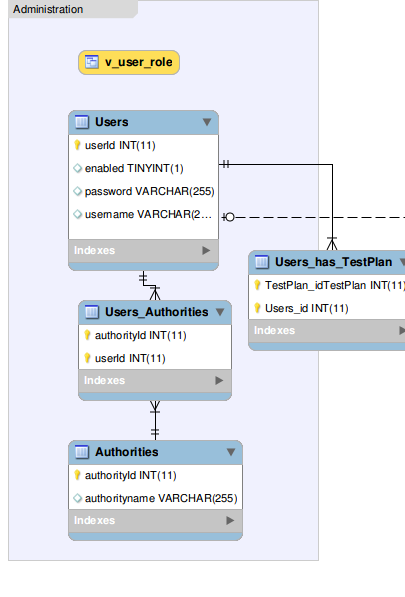
\includegraphics[width=0.3\textwidth]{img/bazaDanychAdministracja.png}  % bez rozszerzenia!
	\caption{Baza danych, część odpowiedzialna za administracje użytkownikami}
	\label{fig:bazaAdmin}
\end{figure}
\subsection{Definicja danych dodatkowych}   

Sekcja ta zawiera encje bazodanowe takie jak: produkt, wydanie produktu, wersja produktu, funkcjonalność, urządzenie, sprzęt. Zdefiniowane encje są łączone w relacji \textit{wiele do wielu} lub \textit{jeden do wielu} podczas tworzenia definicji testu i przy tworzeniu finalnej wersji testu.
   \begin{figure}[h]
\centerline{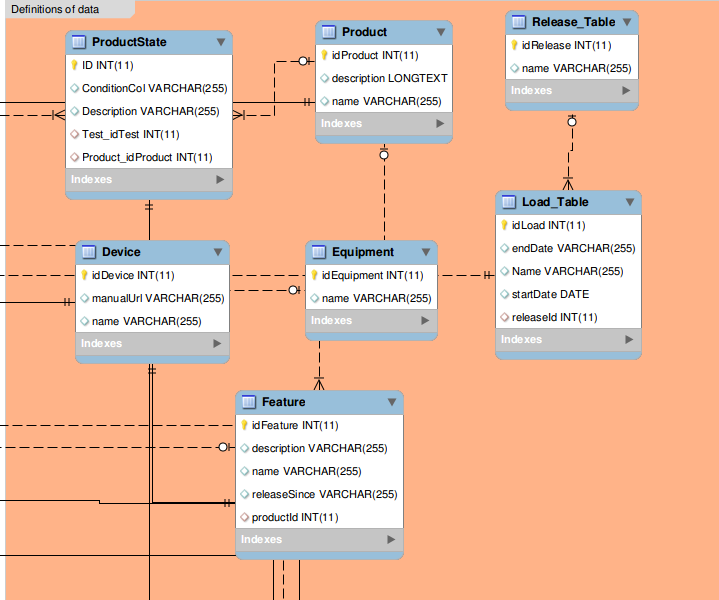
\includegraphics[scale=0.5]{img/bazaDanychDefinicjaDanych.png}}
 \label{fig:bazaDane}
      \caption{Baza danych, część odpowiedzialna za definicje danych dodatkowych}
\end{figure}

 

  
 \subsection{Definicja testów}   
  \begin{figure}
\centerline{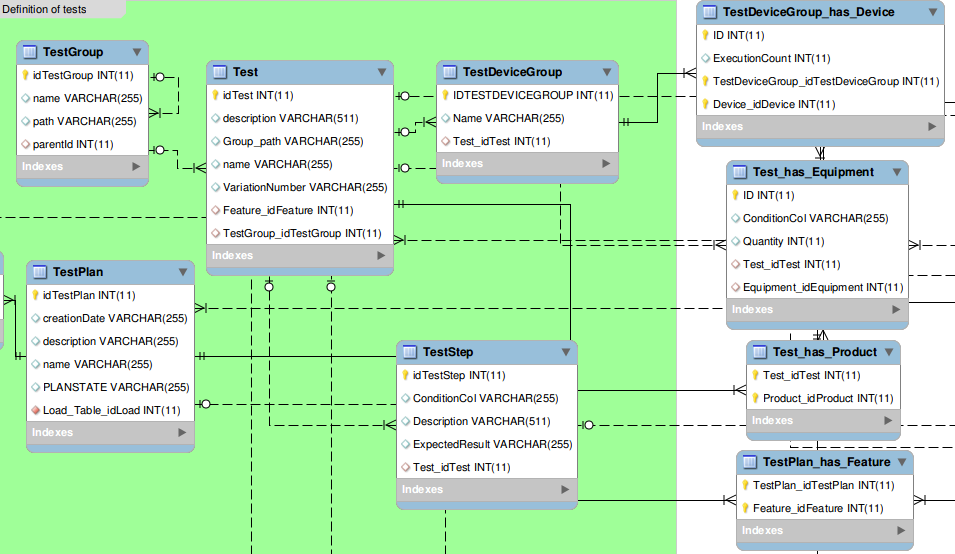
\includegraphics[scale=0.5]{img/bazaDanychDefinicja.png}}
 \label{fig:bazaTesty}
      \caption{Baza danych, część odpowiedzialna za definicje testów}
\end{figure}

 Dla tabel Test i TestGroup zastosowane wzorzec spłaszczonej ścieżki hierarchii\cite{materializedPath} (ang. materialized path). Wzorzec ten pozwala zoptymalizować pobieranie danych dla struktury drzewiastej w bazie danych. Realizacja polega na przypisaniu dla każdego elementu drzewa, pełnej ścieżki począwszy od korzenia :
 \begin{equation}
{idKorzenia}.{idRodzicaPoziomuN}.{idRodzicaPoziomu(N-1)}...{idRodzicaPoziomu1}
\end{equation}
  
  Dzięki takiej strukturze możliwe jest za pomocą jednego zapytania pobranie wszystkich elementów potomnych dla dowolnej ścieżki.
  
  Encje bazodanowe będące składowymi testu zawierają warunki logiczne stanowiące dla jakich urządzeń dla grup urządzeń składowa wchodzi w skład testu. Normalizacja bazy danych sugeruje iż dla przechowywania tego typu warunku należy stworzyć osobną tabelę, która realizuje relacje wiele do wielu dla urządzeń wchodzące w skład warunku. Rozwiązanie takie spowodowałoby jednak podczas pełnego pobrania encji testu, konieczność wykonania kolejnego złączenia (ang. JOIN). Wybrano więc rozwiązanie które dane dotyczące warunku przechowuje w sposób nieznormalizowany w zamian za większą wydajność. Informacje dotyczące warunku po stronie klienckiej (po stronie kodu Java) przechowywane są w tablicy natomiast podczas utrwalania danych tabela ta jest serializowana i składowana jako tekst w jednej kolumnie. Wzorzec ten zastosowany jest dla encji TesthasEquipment, TestStep, ProductState

\subsection{Wykonanie testów} 
Sekcja ta przechowuje testy wykonane lub oczekujące do wykonania przypisane do planów testowych. Podczas przypisania testu do planu należy określić konfigurację urządzeń na której test zostanie wykonany. Informacja ta pozwala na rozwiązanie warunków dla encji których włączenie do definicji testów uwarunkowane jest obecnością określonych urządzeń. Encja wykonania testu zawiera w sobie w relacji jeden do wielu odwołanie do definicji testu. Encje dla których warunek został rozwiązany pozytywnie przypisane są do wykonania testu poprzez relacje wiele do wielu. 
 \begin{figure}[h!]
\centerline{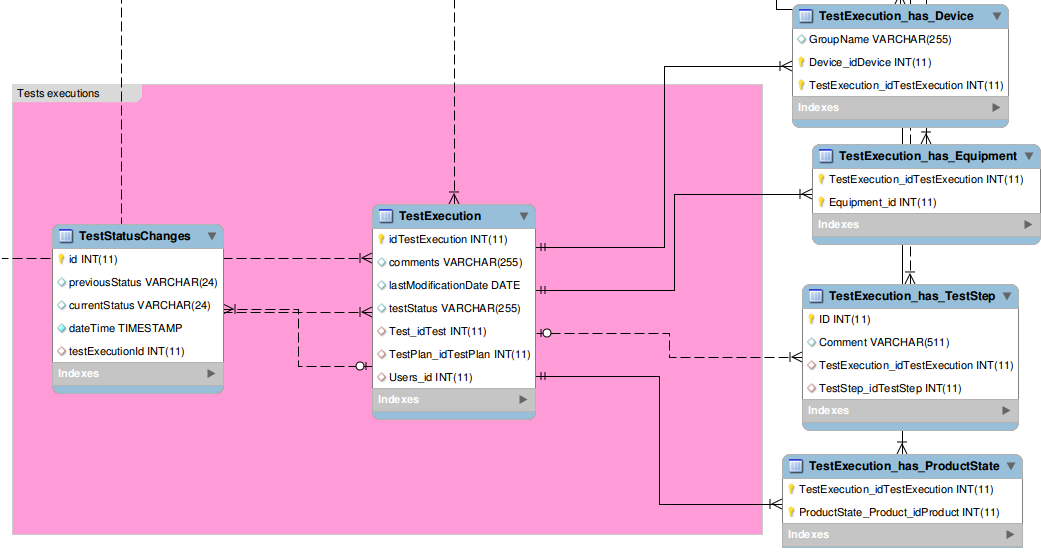
\includegraphics[scale=0.5]{img/bazaDanychWykonanie.png}}
\label{fig:bazaWykonanie}
      \caption{Baza danych, część odpowiedzialna za wykonanie testów}
\end{figure}
Dla relacji pomiędzy wykonaniem testu a pojedynczymi krokami skryptu testowego stworzona została rozszerzona relacja wiele to wielu. Tabela łącząca dla tej relacji zawiera klucze główne dla każdej ze stron relacji i dodatkową kolumnę która przechowuje treść komentarza.

Wykonanie testu podczas cyklu życia zostaje przypisane pod konkretnego użytkownika relacją wiele do jednego. Każda zmiana stanu wykonania testu przez użytkownika przechowywania jest w osobnej tabeli archiwizującej która zawiera historie przejścia między stanami wraz z datą.

\section{Komponenty aplikacji internetowej}

Jak wspomniano w rozdziale dotyczącym projektu aplikacji, warstwa aplikacji internetowej została zrealizowana w technologi JSF przy wykorzystaniu implementacji Mojarra wraz z komponentami dostarczonymi przez bibliotekę PrimeFaces.
W celu wdrożenia aplikacji internetowej na serwerze aplikacji należy zdefiniować plik deskryptora \textit{web.xml}. Konfiguracja dla technologii JSF znajduje się  w pliku \textit{faces-config.xml}, zdefiniowane są tam odwołania do słowników tekstowych które umożliwiają internacjonalizacje aplikacji.

Poniżej przedstawione zostaną składowe pliku \textit{web.xml} związane z konfiguracją aplikacji internetowej pod wymagania technologii JSF

\begin{itemize}
	\item  {\footnotesize \begin{verbatim} <servlet>
        <servlet-name>Faces Servlet</servlet-name>
        <servlet-class>javax.faces.webapp.FacesServlet</servlet-class>
        <load-on-startup>1</load-on-startup>
    </servlet> \end{verbatim}} -- deinicja serwletu
 	\item  {\footnotesize \begin{verbatim}<servlet-mapping>
        <servlet-name>Faces Servlet</servlet-name>
        <url-pattern>/faces/*</url-pattern>
    </servlet-mapping>\end{verbatim}} -- Mapowanie żądań klienta do serwletu
    
    \item  {\footnotesize \begin{verbatim}<context-param>
        <param-name>primefaces.THEME</param-name>
        <param-value>bootstrap</param-value>
    </context-param>\end{verbatim}} -- Ustawienia dotyczące szablonu aplikacji internetowej
\end{itemize}

W powyższym piku konfiguracyjnym określona została ścieżka do implementacja klasy serwletu. Dla technologii JSF klasą implementującą serwlet jest \textit{javax.faces.webapp.FacesServlet}. Następnie wszystkie ścieżki zaczynające się od wzorca \textit{/facet/} zostały przypisane do wyżej zdefiniowanego serwletu. Oznacza to iż dla wszystkich adresów zaczynających się od wzorca \textit{http://adres-aplikacji.org/faces/*}, żądanie zostanie przekazane do serwletu JSF który stworzy i prześlę do przeglądarki wyrenderowaną treść strony.

Określony został również szablon prezentacji graficznej aplikacji internetowej. Parametr \textit{primefaces.THEME} określa który szablon aplikacji powinien zostać załadowany. Użyty został szablon \textit{bootstrap}, jest to szablon który wyglądem zbliżony jest do bazy szablonów warstwy klienckiej \textit{twitter bootstrap}.
\begin{figure}
  \begin{center}
    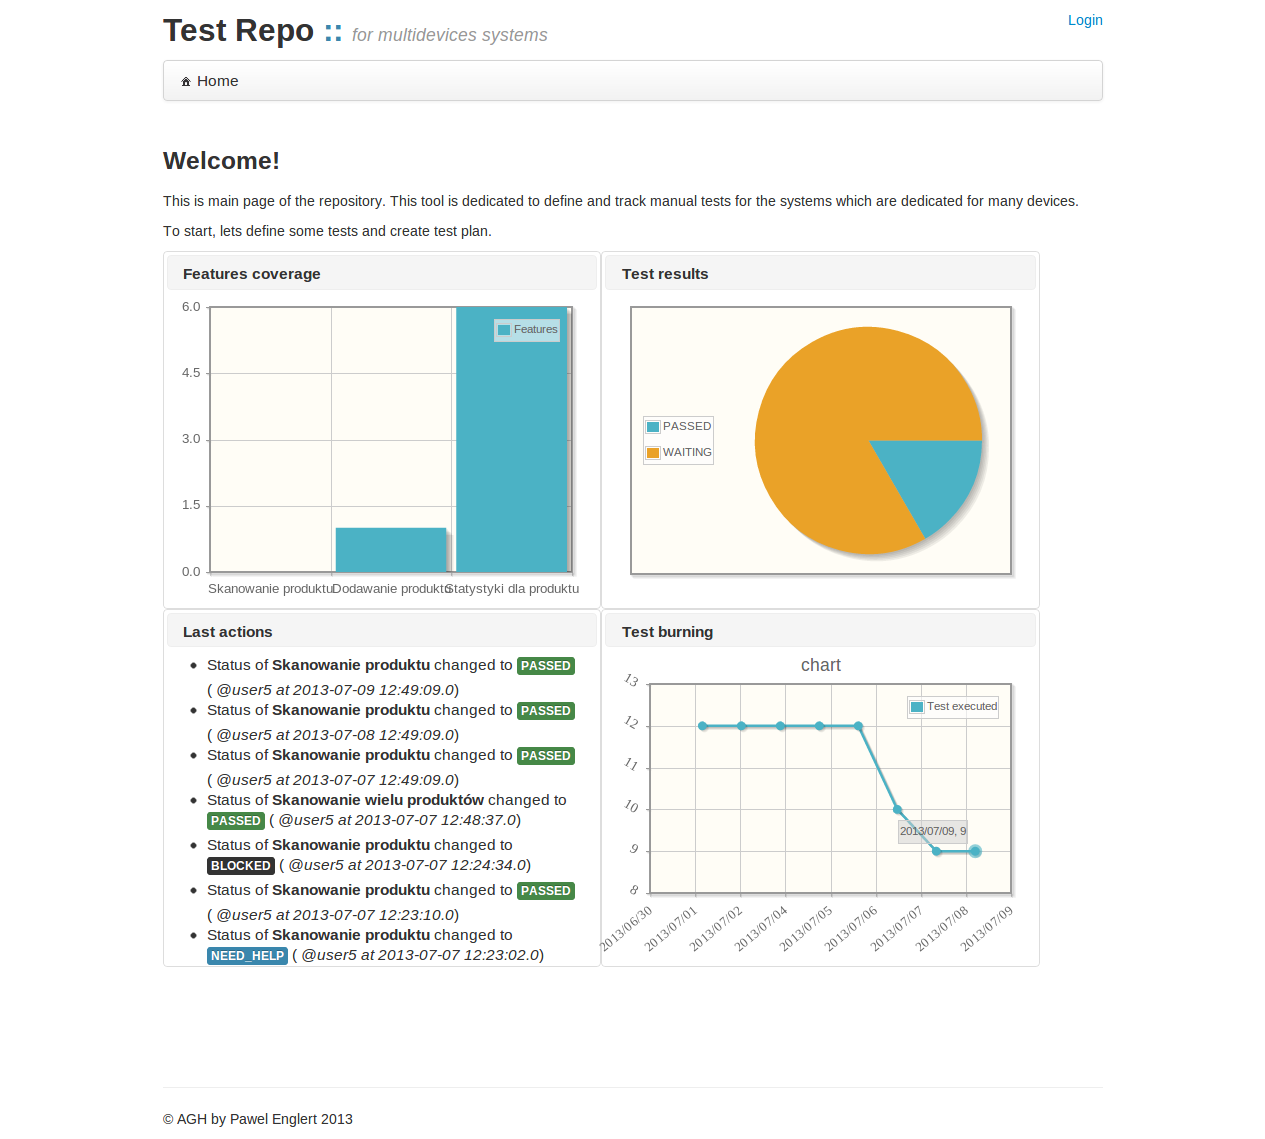
\includegraphics[scale=0.4]{img/screen/Welcome.png}
    \label{fig:stronaGlowna}
    \caption{Strona główna aplikacji internetowej}
  \end{center}
\end{figure}

Zdefiniowane zostały akcje możliwe do wykonania przez użytkownika aplikacji internetowej. Dla każdej z akcji zaprojektowane zostały szablony stron które pozwalają na wykonanie wymienionej akcji. Technologia JSF pozwala na kompozycje szablonów. Stworzony został więc główny szablon strony \textit{index.xhtml}, który zawiera w sobie dwie sekcje: \textbf{tytuł} i \textbf{treść}. Wymienione sekcje rozszerzane są (zapełniane danymi) przez szablony zdefiniowane dla akcji użytkownika.

Plik szablonu dla określonego żądania musi znajdować się na ścieżce wynikającej z adresu żądania. Przykładowo dla żądania \textit{http://adres-aplikacji.org/faces/\textbf{device/index.xhtml}}, wywołany zostanie szablon znajdujący się w lokalizacji \textit{src/main/webapp/\textbf{device/index.xhtml}}.

Kod źródłowy sekcji aplikacji internetowej można podzielić na kilka modułów:
\begin{itemize}
  \item klasy znajdujące się w pakiecie \textbf{edu.agh.repotest.jsf.controller} -- reprezentują kontrolery dla poszczególnych encji, do których dostęp następuje w plikach szablonów
  \item klasy znajdujące się w pakiecie \textbf{edu.agh.repotest.converter} --reprezentują klasy konwertujące obiekty języka JAVA na tekst wyświetlany po stronie warstwy HTML
  \item klasy znajdujące się w pakiecie \textbf{edu.agh.repotest.session} -- reprezentują abstrakcje umożliwiającą operacje na encjach bazodanowych
   
\end{itemize}


\section{Implementacja REST}

Obsługa REST zdefiniowana została w pliku deskryptora (\textit{web.xml}). Zdefiniowany został serwlet obsługujące żądania będące żądaniami do zasobów REST i ustalone zostały wzorce żądania które interpretowane są jako żądania REST. 
\begin{itemize}
	\item  {\footnotesize \begin{verbatim} <servlet>
   <servlet-name>Jersey REST Service</servlet-name>
   <servlet-class>com.sun.jersey.spi.container.servlet.ServletContainer</servlet-class>
        <load-on-startup>1</load-on-startup>
    </servlet> \end{verbatim}} -- deinicja serwletu obsługującego żądania REST
 	\item  {\footnotesize \begin{verbatim}<servlet-mapping>
        <servlet-name>Jersey REST Service</servlet-name>
        <url-pattern>/rest/*</url-pattern>
    </servlet-mapping>\end{verbatim}} -- Mapowanie żądań do zasobów REST, wszystkie żądania zaczynające się od wzorca \textit{rest}
  \end{itemize}
  
  
  Kod źródłowy języka JAVA zawiera klasy kontrolerów (w pakiecie \textbf{edu.agh.repotest.rest}) dla których przypisane są wzorce żądania do zasobu. Mapowanie między adresem zasobu a kontrolerem odbywa się poprzez zastosowanie adnotacji które określają wzorzec dostępu do zasobu i typ żądania. Na potrzeby usługi internetowej stworzono encje z adnotacjami JAXB które mogą być serializowane do postaci XML i JSON. Encje te są rodzajem adaptera na encjach bazodanowych.
  \newpage
  
  
 \begin{lstlisting}[caption=Pobranie testów do wykonania dla użytkownika,label=lst:pobranieTestow]

@Stateless
@Path("/users")
public class Users {

    @GET
    @Path("{username}/testsExecutions")
    @Produces({MediaType.APPLICATION_ATOM_XML, MediaType.APPLICATION_JSON})
    public List<edu.agh.repotest.dao.TestExecution> showTestsForUser(@PathParam("username") String username) {
        /*
          body of the method
        */
    }

\end{lstlisting}
 
 Kod źródłowy \ref{lst:pobranieTestow} ilustruje sytuacje gdy adres żądania \textit{http://adres-aplikacji.org/rest/\textbf{users/user1/testExecutions}} wyświetli listę testów dla użytkownika \textit{user1} w postaci XML lub JSON. Adnotacja na poziomie klasy określa początek adresu (\textit{users}), adnotacja na poziomie metody określa iż dopasowany zostania ciąg znaków .*/testsExecutions, przy czym pierwszy człon adresu przekazany zostanie do metody jako argument username. Adnotacja GET określa iż metoda zostanie wywołana jedynie w przypadku odwołania się poprzez metodę \textit{GET} dla protokołu \textit{HTTP}. Adnotacja \textit{Produces} określa w jakim formacie zwrócone zostaną dane. Końcowy format negocjowany jest z klientem wywołującym żądanie który przesyła w nagłówku jaki format jest przez niego preferowany.
 
Poniżej przedstawione zostaną stworzone mapowania dla zasobów:
\begin{itemize}
  \item users \textbf{[GET]} -- wyświetla wszystkich użytkowników
  \item users/{$username$} \textbf{[GET]} -- wyświetla informacje o użytkowniku
  \item users/{$username$}/testExecutions \textbf{[GET]}-- wyświetla testy przypisane dla użytkownika
  \item testExecutions/{$id$} \textbf{[GET]} -- wyświetla informacje o teście do wykonania
  \item testExecutions/{$id$} \textbf{[POST]}-- modyfikuje test
  \item features \textbf{[PUT]} -- dodaje funkcjonalność
  
\end{itemize}


